%&../.preamble
\endofdump

\usetikzlibrary {er}
\usetikzlibrary{external}
\usetikzlibrary{patterns}
\tikzset{external/system call={pdflatex --shell-escape --fmt=../.preamble --halt-on-error -jobname "\image" "\endofdump\texsource"}}
\tikzexternalize[prefix=tikz/]

\title{Basi di dati}
\author{Marini Mattia}
\date{$ 1^o $ semestre $ 2^o $ anno}

\begin{document}
\maketitle
\tableofcontents
\newpage

\section{Introduzione}
Per immagazzinare dati abbiamo bisogno di:
\begin{itemize}
	\item \underline{Base di dati} raccolta organizzata  di informazioni
	\item \underline{Database Managment System} o DBMS: pacchetto software per gestire basi di dati
\end{itemize}
L'insieme di base di dati e DBMS è detto \underline{database system}
\vskip3mm
Un DBMS deve fornire come minimo:
\begin{itemize}
	\item \underline{Data Definition Language (DDL)} ossia un linguaggio che permetta di definire la struttura dei dati
	\item \underline{Data Manipulationn Language (DML)} o quey language, che permetta di modificare ed estrarre i dati
	\item Garantire \underline{robustezza} dei dati, rendendo possibile il recupero in caso di corruzione
	\item Gestire problemi di \underline{concorrenza}:
	      \begin{itemize}
		      \item Evitare interazioni indesiderate tra utenti \textit{isolation}
		      \item Evitare modifiche incomplete dei dati \textit{atomicity}
	      \end{itemize}
\end{itemize}
\subsubsection*{Vantaggio database}
Utilizzare un database comporta molti vantaggi. Uno dei più importanti è che permette la \underline{separazione tra programmi e dati}
\vskip3mm
Devo modificare lo schema fisico secondo il quale salvo i dati
\vskip3mm
\begin{minipage}[t]{0.48\textwidth}
	\begin{center}
		Database
	\end{center}
	\begin{itemize}
		\item Modifico database, ma modalità logiche secondo le quali accedo e modifico dati rimangono le stesse
		\item Applicazione \underline{non deve essere modificata}
	\end{itemize}
\end{minipage}
%
\begin{minipage}[t]{0.48\textwidth}
	\begin{center}
		Salvataggio su file
	\end{center}
	\begin{itemize}
		\item La struttura del file è memorizzata nel programma
		\item Cambio struttura file
		\item Applicazione \underline{deve essere modificata}
	\end{itemize}
\end{minipage}
\vskip3mm
Dunque il salvataggio su file rende manutenzione difficile e costosa
\subsubsection*{Livelli di astrazione}
\begin{itemize}
	\item Schema fisico: fornisce dettagli su come i dati sono salvati fisicamente nella memoria
	\item Schema concettuale: modello di alto livello che rappresenta i dati nei termiini del modello del DBMS
	\item Schema esterno: permette di creare una o più vistte per interfacciarsi con il database
\end{itemize}
\begin{center}
	\begin{forest}
		for tree={draw, grow = 90}
		[Disk
			[Schema fisico
					[Schema concettuale
							[Schema esterno 1]
							[Schema esterno 2]
							[Schema esterno 3]
					]
			]
		]
	\end{forest}
\end{center}
\subsubsection*{Attori sulla scena}
\begin{itemize}
	\item  \underline{Database administrator}: monitora utilizzo DB, regola accesso, acquista risose hardware e monitora efficienza
	\item \underline{Database designer}: crea il design del DB, definendone lo schema e i vincoli sulle transaioni
\end{itemize}
Utenti finali (utilizzatori database):
\begin{itemize}
	\item  \underline{Casual}: "accedono da esperti", ma occasionalmente, quando necessario
	\item \underline{Naive}
	      \begin{itemize}
		      \item Utilizzano funzioni predefinite
		      \item Es. cassiedi di banca, impiegati, utenti di siti web...
	      \end{itemize}
	\item \underline{Sophisticated}: business analysts, data scientists, ingegneri. Utilizzano software molto vicini a quello della base di dati
	\item \underline{Stand-alone}: utenti che si creano una base di dati "per conto loro", ad esempio un commercialista che si crea un database con i dati dei suoi clienti
\end{itemize}
\section{Progettazione di una base di dati}
Le fasi della progettazione di una base di dati sono le seguenti:
\begin{itemize}
	\item Fasi principali
	      \begin{itemize}
		      \item Analisi dei requisiti
		      \item Progettazione concettuale
		      \item Progettazione logica
	      \end{itemize}
	\item Fasi seconda parte
	      \begin{itemize}
		      \item Raffinamento dello schema logico (normalizzazione)
		      \item Progettazione del livello fisico
		      \item Progettazione applicativa e sicurezza
	      \end{itemize}
\end{itemize}

\subsection{Concetti base modellazione logica}
\subsubsection*{Entità}
\begin{itemize}
	\item Un'entità è un \underline{oggetto singolo} del mondo reale. Ad esempio Mario
	\item Un entity set è un insieme di entità, quindi ad esempio il gruppo di amici Mario, Paolo e Nicola
	\item Un entity type è il \underline{tipo generico di entità}, ad esempio Persona
\end{itemize}
Un'entity è rappresentata tramite un quadrato nei diagrammi:
\begin{center}
	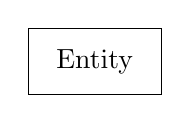
\begin{tikzpicture}
		\node (Entity)[entity] at (0,0) {Entity};
	\end{tikzpicture}
\end{center}

\subsubsection*{Attributi}
\begin{itemize}
	\item Un attribute è una proprietà usata per descrivere un'entity. Ad esempio, mario avrà codice fiscale, numero telefono...
	\item Un value set o data type è la variabile che contiene il valore dell'attributo
\end{itemize}
Gli attributi possono essere \underline{semplici, composti e multi valore}. Noi useremo quelli semplici e basta. Possiamo ricreare gli altri tramite diversi workarround
Un'entity è rappresentata tramite un ovale nei diagrammi:
\begin{center}
	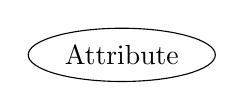
\begin{tikzpicture}
		\node (Entity)[attribute] at (0,0) {Attribute};
	\end{tikzpicture}
\end{center}

L'attributo viene collegato all'entity type al quale fa riferimento
\begin{center}
	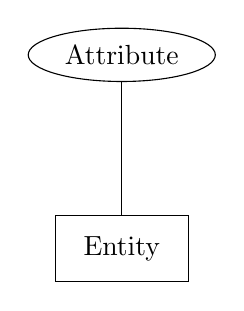
\begin{tikzpicture}[node distance = 7 em]
		\node (Entity)[entity] at (0,0) {Entity};
		\node ()[attribute, above of = Entity] {Attribute} edge (Entity);
	\end{tikzpicture}
\end{center}



\subsubsection*{Attributo chiave}
Un attributo chiave è un attributo che \underline{identifica in maniera univoca} l'entità alla quale fa riferimento. Ad esempio, l'isbn di un libro. La chiave primaria va sempre sottolineata:
\begin{center}
	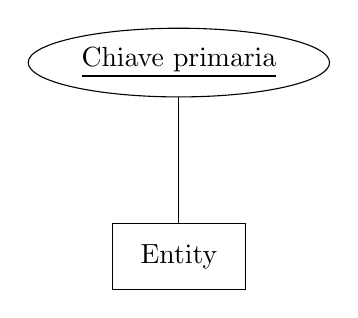
\begin{tikzpicture}[node distance = 7 em]
		\node (Entity)[entity] {Entity};
		\node [attribute, above of = Entity] {\underline{Chiave primaria}} edge (Entity);
	\end{tikzpicture}

	Una chiave può essere inoltre
	\begin{itemize}
		\item Composta, ossia formata da più attributi. Ad esempio, nome e matricola
		\item Multipla, ossia vi sono più \underline{chiavi candidate}, ad esempio la targa e il numero di telaio di un'automobile. Va sempre comunque indicata la \underline{chiave principale}
	\end{itemize}
\end{center}

\subsubsection*{Relazioni}
Una relazione è un'associazione tra due o più entity

\begin{center}
	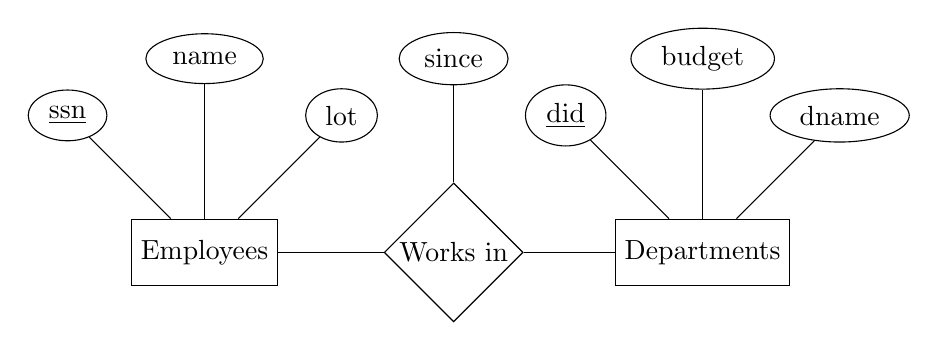
\begin{tikzpicture}[ node distance =7 em]
		\node (Employees)[entity] at (0,0) {Employees};
		\node (name)[attribute, above of = Employees]  {name} edge (Employees);
		\node (ssn)[attribute, above left of = Employees]  {\underline{ssn}} edge (Employees);
		\node (lot)[attribute, above right of = Employees]  {lot} edge (Employees);
		\node (Works in)[relationship, right of = Employees, xshift = 20pt] {Works in} edge (Employees);
		\node (since)[attribute, above of = Works in] {since} edge (Works in);
		\node (Departments)[entity, right of = Works in, xshift = 20pt] {Departments} edge (Works in);
		\node (did)[attribute, above left of = Departments] {\underline{did}}edge (Departments) ;
		\node (dname)[attribute, above right of = Departments] {dname}edge (Departments);
		\node (budget)[attribute, above of = Departments] {budget}edge (Departments);
	\end{tikzpicture}
\end{center}

Una relazione può essere anche a 3 (uwu)
\begin{center}
	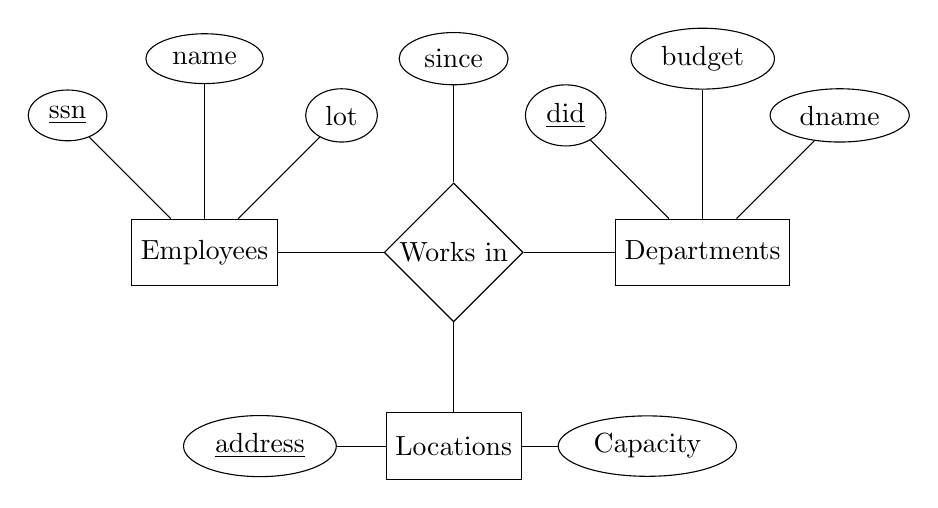
\begin{tikzpicture}[ node distance =7 em]
		\node (Employees)[entity] at (0,0) {Employees};
		\node (name)[attribute, above of = Employees]  {name} edge (Employees);
		\node (ssn)[attribute, above left of = Employees]  {\underline{ssn}} edge (Employees);
		\node (lot)[attribute, above right of = Employees]  {lot} edge (Employees);
		\node (Works in)[relationship, right of = Employees, xshift = 20pt] {Works in} edge (Employees);
		\node (since)[attribute, above of = Works in] {since} edge (Works in);
		\node (Departments)[entity, right of = Works in, xshift = 20pt] {Departments} edge (Works in);
		\node (did)[attribute, above left of = Departments] {\underline{did}}edge (Departments) ;
		\node (dname)[attribute, above right of = Departments] {dname}edge (Departments);
		\node (budget)[attribute, above of = Departments] {budget}edge (Departments);
		\node (Locations)[entity, below of = Works in] {Locations} edge (Works in);
		\node (address)[attribute, left of = Locations] {\underline{address}} edge (Locations);
		\node (Capacity)[attribute, right of = Locations] {Capacity}edge (Locations);
	\end{tikzpicture}
\end{center}

\subsection{Vicoli di relazione}
Spesso abbiamo bisogno di specificare qualche vincolo riguardo ad una relationship tra due entity
\subsubsection*{Vincolo di chiave}
Si rappresenta con una freccia:
\begin{center}
	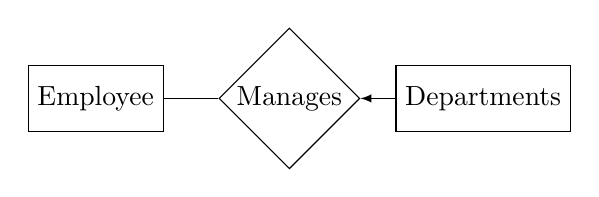
\begin{tikzpicture}[node distance = 7 em]
		\node (Employee)[entity] {Employee};
		\node (Manages)[relationship, right of = Employee] {Manages}edge (Employee);
		\node (Departments)[entity, right of = Manages] {Departments}edge[-latex] (Manages);
	\end{tikzpicture}
\end{center}
In questo caso significa che \underline{ogni dipartimento può avere \textbf{al più} un manager}

\subsubsection*{Vincolo di partecipazione }
Si rappresenta con una linea grossa:
\begin{center}
	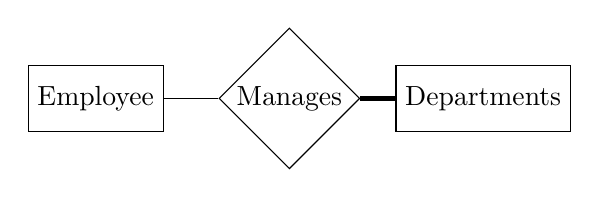
\begin{tikzpicture}[node distance = 7 em]
		\node (Employee)[entity] {Employee};
		\node (Manages)[relationship, right of = Employee] {Manages}edge (Employee);
		\node (Departments)[entity, right of = Manages] {Departments}edge[line width = 0.6mm] (Manages);
	\end{tikzpicture}
\end{center}
In questo caso significa che \underline{ogni dipartimento deve avere \textbf{almeno} un manager}
\vskip3mm
I vincoli di chiave e di partecipazione possono essere uniti, come segue:
\begin{center}
	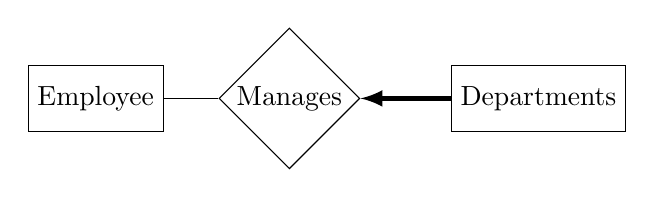
\begin{tikzpicture}[node distance = 7 em]
		\node (Employee)[entity] {Employee};
		\node (Manages)[relationship, right of = Employee] {Manages}edge (Employee);
		\node (Departments)[entity, right of = Manages, xshift = 20pt] {Departments}edge[-latex, line width = 0.6mm] (Manages);
	\end{tikzpicture}
\end{center}
In questo caso significa che \underline{ogni dipartimento ha \textbf{esattamente} uno e uno solo manager}

\subsubsection*{Esempio completo}
\begin{center}
	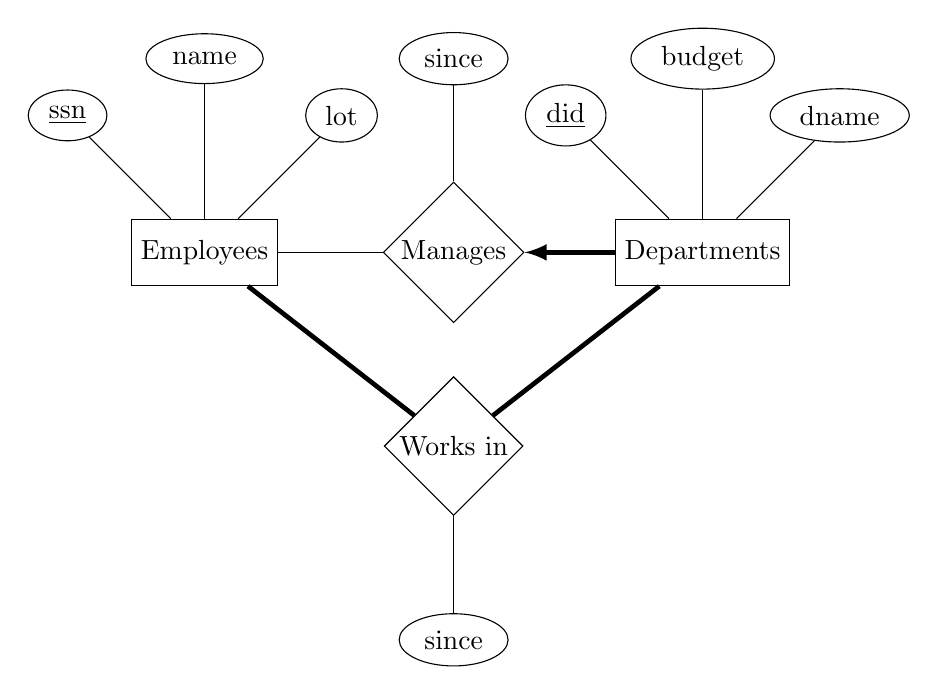
\begin{tikzpicture}[ node distance =7 em]
		\node (Employees)[entity] at (0,0) {Employees};
		\node (name)[attribute, above of = Employees]  {name} edge (Employees);
		\node (ssn)[attribute, above left of = Employees]  {\underline{ssn}} edge (Employees);
		\node (lot)[attribute, above right of = Employees]  {lot} edge (Employees);
		\node (Manages)[relationship, right of = Employees, xshift = 20pt] {Manages} edge (Employees);
		\node (since)[attribute, above of = Manages] {since} edge (Manages);
		\node (Departments)[entity, right of = Manages, xshift = 20pt] {Departments} edge[-latex, line width = 0.6mm] (Manages);
		\node (did)[attribute, above left of = Departments] {\underline{did}}edge (Departments) ;
		\node (dname)[attribute, above right of = Departments] {dname}edge (Departments);
		\node (budget)[attribute, above of = Departments] {budget}edge (Departments);
		\node (Works in)[relationship, below of = Manages] {Works in} edge [line width = 0.6mm](Employees) edge[line width = 0.6mm] (Departments);
		\node (since)[attribute, below of = Works in] {since} edge (Works in);
	\end{tikzpicture}
\end{center}

\subsubsection*{Notazione (min, max)}
Una notazione alternativa per esprimere dei vincoli sul numero di entity coinvolte nella relazione è utilizzare un disegno come segue:
\begin{center}
	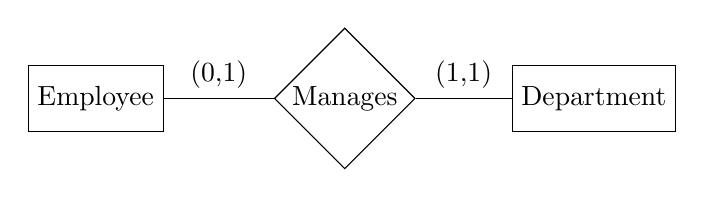
\begin{tikzpicture}[node distance = 7 em]
		\node (Employee)[entity] {Employee};
		\draw node (Manages)[relationship, right of = Employee, xshift = 20 pt] {Manages};
		\node (Department)[entity, right of = Manages, xshift = 20 pt] {Department};
		\draw (Employee)--(Manages) node [midway, above] {(0,1)};
		\draw (Manages)--(Department) node [midway, above] {(1,1)};
	\end{tikzpicture}
	\vskip3mm
	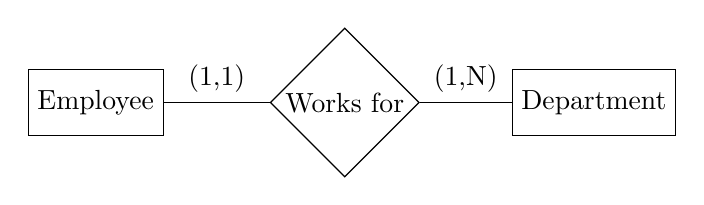
\begin{tikzpicture}[node distance = 7 em]
		\node (Employee)[entity] {Employee};
		\draw node (Manages)[relationship, right of = Employee, xshift = 20 pt] {Works for};
		\node (Department)[entity, right of = Manages, xshift = 20 pt] {Department};
		\draw (Employee)--(Manages) node [midway, above] {(1,1)};
		\draw (Manages)--(Department) node [midway, above] {(1,N)};
	\end{tikzpicture}
\end{center}
\vskip3mm
Nel primo caso si legge: un Employee può essere manager di 0 o 1 department. Un department può essere gestito da un solo manager
\subsubsection*{Gerarchie di classi}
Come usiamo la generalizzazioe all'interno dei class diagrams, possiamo utilizzarla nei diagrammi er
\begin{center}
	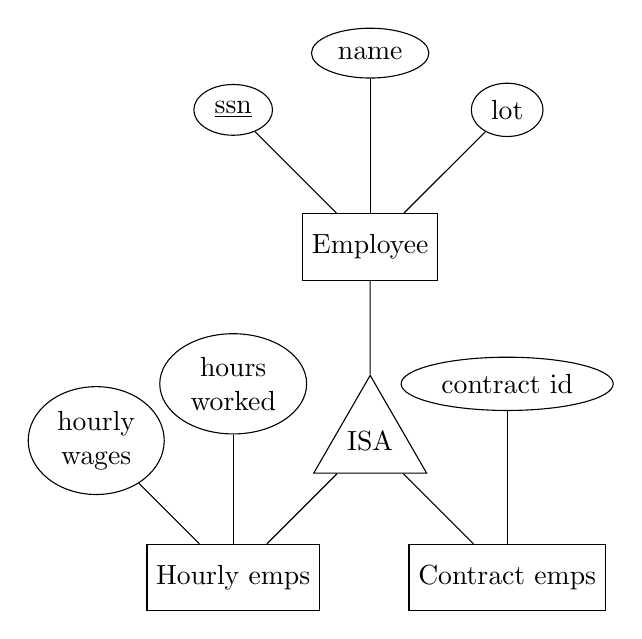
\begin{tikzpicture}[node distance = 7 em]
		\node (Employee)[entity] {Employee};
		\node (ssn)[attribute, above left of = Employee] {\underline{ssn}};
		\node (name)[attribute, above of = Employee] {name};
		\node (lot)[attribute, above right of = Employee] {lot};
		\node (ISA)[regular polygon, regular polygon sides=3, draw, inner sep = 0, fill = white, below of = Employee]  {ISA};
		\node (Hourly emps)[entity, below left of = ISA] {Hourly emps};
		\node (Contract emps)[entity, below right of = ISA] {Contract emps};
		\node (contract id)[attribute, above of = Contract emps] {contract id};
		\node (hours worked)[attribute, above of = Hourly emps, align = center] {hours\\worked};
		\node (hourly wages)[attribute, above left of = Hourly emps, align = center] {hourly\\wages};
		%
		\draw (Hourly emps)edge (hours worked) edge (hourly wages);
		\draw (Contract emps)--(contract id);
		\draw (ISA)edge (Employee) edge (Hourly emps) edge (Contract emps);
		\draw (Employee)edge(ssn) edge (name) edge (lot);
	\end{tikzpicture}
\end{center}

In questo casi si dice che:
\begin{itemize}
	\item \verb|Hourly emps| e \verb|Contract emps| sono \underline{generalizzati} in \verb|Employee|
	\item \verb|Employee| si specializza con \verb|Contract emps| e \verb|Hourly emps|
\end{itemize}
Inoltre possiamo rappresentare i seguenti concetti di \underline{overlap e copertura} secondo i seguenti schemini grafici
\vskip5mm
\begin{minipage}[t]{0.48\textwidth}
	\begin{center}
		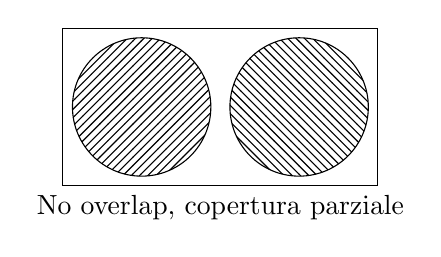
\begin{tikzpicture}
			\draw  (0,0) rectangle (4,2);
			\draw [pattern = north east lines](1,1)circle [radius = 25pt];
			\draw [pattern = north west lines](3,1)circle [radius = 25pt];
			\node [below] at (2,0) {No overlap, copertura parziale};
		\end{tikzpicture}
	\end{center}
	\begin{center}
		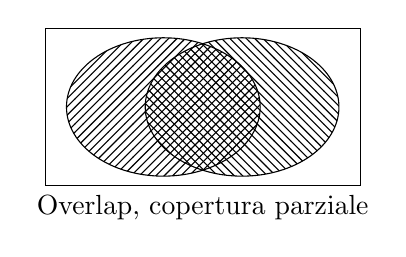
\begin{tikzpicture}
			\draw  (0,0) rectangle (4,2);
			\draw [pattern = north east lines](1.5,1)circle [y radius = 25pt, x radius = 35pt];
			\draw [pattern = north west lines](2.5,1)circle [y radius = 25pt, x radius = 35pt];
			\node [below] at (2,0) {Overlap, copertura parziale};
		\end{tikzpicture}
	\end{center}
\end{minipage}
%
\begin{minipage}[t]{0.48\textwidth}
	\begin{center}
		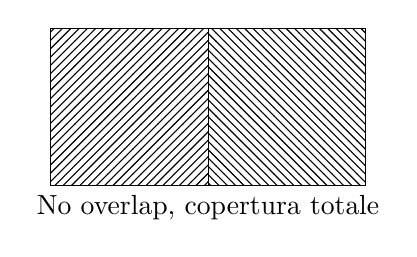
\begin{tikzpicture}
			\draw  (0,0) rectangle (4,2);
			\draw [pattern = north east lines](0,0)rectangle(2,2);
			\draw [pattern = north west lines](2,0)rectangle(4,2);
			\node [below] at (2,0) {No overlap, copertura totale};
		\end{tikzpicture}
	\end{center}

	\begin{center}
		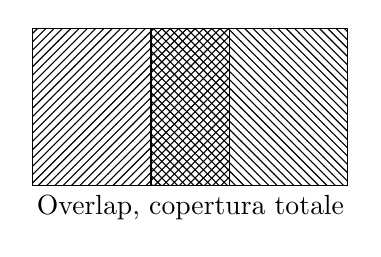
\begin{tikzpicture}
			\draw  (0,0) rectangle (4,2);
			\draw [pattern = north east lines](0,0)rectangle(2.5,2);
			\draw [pattern = north west lines](1.5,0)rectangle(4,2);
			\node [below] at (2,0) {Overlap, copertura totale};
		\end{tikzpicture}
	\end{center}
\end{minipage}
\vskip5mm

\subsubsection*{Aggregazione}
\section{Riassuntone}
\subsection{Termini}
\begin{itemize}
	\item \underline{Superchiave}: un insieme di attributi che identifica univocamente una tupla
	\item \underline{Superchiave minimale}: superchiave che se si toglie uno qualsiasi degli attributi non è più chiave
	\item \underline{Chiavi candidate}: tutte le superchiavi minimali di una relazione
	\item \underline{Attributo primot}: attributo che appartiene \underline{almeno} ad una chiave candidata
	\item \underline{Attributo non primot}: attributo che non appartiene \underline{a nessuna} chiave candidata
	\item \underline{Schema (scheme)}: insieme di tabelle e vincoli di integrità di un db
\end{itemize}
\subsection{Vincoli}
\begin{itemize}
	\item Dominio: il tipo inserito in una colonna deve rispettare il formato della colonna stessa:
	      \begin{itemize}
		      \item Data type \textit{\textit{string, int,...}}
		      \item Range (\textit{int in range 0-120})
		      \item Format (\textit{mail, contains "@"})
		      \item Enum values (\textit{value can be either a,b,c,...})
		      \item Null constrait (\textit{Item cannot be null})
	      \end{itemize}
	\item Chiave: deve esistere una chiave per ogni relazione
	\item Integrità delle entità: nessun valore della chiave primaria può essere null
	\item Integrità referenziale: una foreign key non può far riferimento ad una tupla non presente nella relazione referenziata
	\item Vincoli di integrità semantica: vincoli che non possono essere espressi dal dbms stesso (\textit{es, tutti gli impiegati non possono lavorare più di 46 ore a settimana})
\end{itemize}
\subsubsection*{Violazione dei vincoli}
\begin{itemize}
	\item \underline{Insert}: viola tutti:
	      \begin{itemize}
		      \item Dominio (valore con tipo sbagliato)
		      \item Integrità entità (chiave null)
		      \item Integrità referenziale (Fk non esiste)
		      \item Integrità semantica
	      \end{itemize}
	\item \underline{Delete}
	\item Integrità referenziale (toglie valore referenziato )
	\item \underline{Update}: viola tutti:
	      \begin{itemize}
		      \item E' come delete + insert
	      \end{itemize}
\end{itemize}
\subsubsection*{Mantenere integrità}
\begin{itemize}
	\item \underline{Restrict}: impedisce operazione
	\item \underline{Cascade}: rimuove tuple che referenziano tupla eliminata
	\item \underline{Set null/default}: setta la chiave referenziante a nulla/default value
\end{itemize}
\subsection{Mapping}
\begin{itemize}
	\item \underline{Vincolo di chiave} ($ E_1, E_2 $, vincolo su $ E_2 $ )
	      \begin{itemize}
		      \item Opzione 1: $ FK\left(E_1, E_2\right), PK\left(E_2\right) $
		      \item Opzione 2: aggiungo colonna a $ E_2 $ che referenzia $ PK\left(E_1\right) $
	      \end{itemize}
	\item \underline{Vincolo di partecipazione totale} ($ E_1, E_2 $, vincolo su $ E_2 $): non può essere rappresentato completamente, ma solo in parte
	      \begin{itemize}
		      \item Aggiungo \textit{not null} sulla $ FK\left(E_1\right) $ in $ E_2 $
	      \end{itemize}
	\item \underline{Weak entities} ($ E_1, E_2 $, $ E_2 $ è weak)
	      \begin{itemize}
		      \item $ FK\left(E_2\right) $ è \textit{not null} (attributo non esiste senza istanza padrone)
		      \item ON DELETE CASCADE per eliminare weak instance quando viene eliminata estanza padrone
	      \end{itemize}
	\item \underline{Gerarchie IS-A} ($ E, C_1, C_2 $):
	      \begin{itemize}
		      \item Opzione 1:
		            \begin{itemize}
			            \item $ PK(E) = \text{ ssn }$  $ PK\left(C_1\right) = FK\left(C_1\right) = \text{ ssn } $ e estessa cosa per $ C_2 $
			            \item ON DELETE CASCADE: se elimino superclasse elimino anche classe child corrispondente
		            \end{itemize}
		      \item Opzione 2 (se ce copertura totale): elimino classe padre
	      \end{itemize}
	\item \underline{Aggregazioni}: Relazione esterna ha attributi della relazione interna e la chiave di ciò a cui è collegata. Si può semplificare se
	      \begin{itemize}
		      \item Relazione esterna non ha attributi
		      \item Aggregazione ha vincolo di partecipazione totale su relazione esterna
	      \end{itemize}
\end{itemize}
\subsection{Algebra relazionale}
\begin{itemize}
	\item $ \sigma  $: select
	\item $ \pi  $ : project
	\item $ \rho  $: rename
	\item Divisione: $ A\left(x, y\right) / B\left(y\right) $
	      \begin{itemize}
		      \item Raggruppo per colonne $ x $ di $ A $
		      \item Metto in tabella risultato gli $ x $ che hanno tutti gli y di $ A $
		            \[
			            A / B = \left\{x \text{ t.c. } \exists \left<x,y\right> \forall y \in B \right\}
		            \]
	      \end{itemize}
\end{itemize}
\subsection{Normalizzazione}
\begin{itemize}
	\item \textbf{Prima forma normale}:
	      \begin{itemize}
		      \item No attributi multivalore
		      \item No tuple duplicate (esiste chiave)
	      \end{itemize}
	\item \textbf{Seconda forma normale}: no dipendenze parziali
	      \begin{itemize}
		      \item Controlla che tutti gli attributi non primi non dipenda parzialmente da alcuna chiave candidata
	      \end{itemize}
	      \textbf{Terza forma normale}: no dipendenze transitive. Per ogni dipendenza funzionale, $ X \rightarrow Y $
	      \vskip3mm
	      Ogni freccia entrante in un attributo non primo deve dipendere da una chiave candidata
	      \begin{itemize}
		      \item $ X $ è superchiave
		      \item $ Y $ è primo
	      \end{itemize}
	\item \textbf{Forma di Boyce Codd}
	      \begin{itemize}
		      \item Per ogni df $ X \rightarrow Y $, X deve essere una superchiave
	      \end{itemize}
\end{itemize}

\subsection{Livello fisico}
\subsubsection*{Terminologia}
\begin{itemize}
	\item $ P $: dimensione della pagina
	\item $ S: $ dimensione del file
	\item $ t_R $ dimensione di una tupla di una tabella $ R $
	\item $ P_R $: numero di pagine che contengono tuple di $ R $
	\item $ \left|R.A\right| $: numero di valori diversi per l'attributo $ A $
	\item $ \left|R\right| $: numero di tuple di $ R $
	\item $ \left|R_{c==c}\right| $: numero di tuple per le quali è soddisfatta la condizione c == c
	\item $ f= \frac{1}{\left|R.A\right|} $: selectivity factor
\end{itemize}

\subsubsection*{Heap list}
\begin{itemize}
	\item Scan
	      \[
		      P_R
	      \]
	\item Equality search
	      \[
		      P_R
	      \]
	\item Insert
	      \[
		      2
	      \]
	      leggo ultima pagina in $ \frac{S}{P}-1 $ e eventualmente ne aggiungo una nuova
	\item Delete
	      \[
		      P_R + \left|R_{c=c}\right| \quad \text{ dove } \left|R_{c=c}\right| \approx \frac{\left|R\right|}{\left|R.A\right|}
	      \]
\end{itemize}

\subsubsection*{Sorted file}
\begin{itemize}
	\item Scan:
	      \[
		      P_R
	      \]
	\item Equality search o ricerca per intervallo:
	      \[
		      \log_2\left(P_R\right) + \left\lceil \frac{\left|R_{c=c}\right|}{\frac{P}{t_R}} \right\rceil
	      \]
	\item Delete:
	      \[
		      \log_2\left(P_R\right) + 2 \cdot \left\lceil \frac{\left|R_{c=c}\right|}{\frac{P}{t_R}} \right\rceil
	      \]
	      il $ \cdot 2 $ è dato dal fatto che le pagine contenenti le tuple vanno prima lette e poi eliminate
	\item Insert
	      \[
		      \log_2\left(P_R\right) + 1
	      \]
	      Se non c'è spazio ho bisogno di spostare tutte le $ P_R $ tuple nel caso peggiore
\end{itemize}

\subsubsection*{B+ tree}
Costo lookup:
\[
	\log_B \left(R.A\right)
\]
Equality search unclustered (nel caso peggiore ogni tupla sta in una pagina diversa):
\[
	\log_B \left(R.A\right) + R_{a = a}
\]
Equality search clustered (tuple sono contigue quindi complessità diminuisce):
\[
	\log_B \left(R.A\right) +\left\lceil \frac{\left|R_{a = a}\right|}{ \frac{P}{t_r}} \right\rceil
\]
Insert:
\[
	\log_B \left(R.A\right)  + 2
\]
\subsubsection*{Hash table}
Costo lookup:
\[
	L_h \approx 1.2
\]
Costo insert:
\[
	L_h + 2
\]


\subsection{Joins}
\subsubsection*{Nested Loop Join}
\[
	P_R  \cdot  \left(P_S + 1\right)
\]
\subsubsection*{Sort Merge Join}
Costo se tuple già ordinate:
\[
	P_R + P_S
\]
Costo ordinamento tuple:
\[
	2 \cdot  P_R \cdot  \left(\left\lceil \log_{b-1} \left\lceil \frac{P_R}{B} \right\rceil \right\rceil + 1\right)
\]
\subsubsection*{Hash join}
Costo se tuple già in bucket:
\[
	P_R + P_S
\]
Costo inserimento in bucket:
\[
	P_R + 2 \cdot \left|R\right|
\]
\subsubsection*{Indexed Nested Loop Join}
\[
	P_R + \left|R\right| \cdot  \text{ CostoEqualitySearch }
\]

\end{document}
